%  The AAU Poster Theme.
%  2013-05-08 v. 1.1.0
%  Copyright 2013 by Jesper Kjær Nielsen <jkn@es.aau.dk>
%
%  This is free software: you can redistribute it and/or modify
%  it under the terms of the GNU General Public License as published by
%  the Free Software Foundation, either version 3 of the License, or
%  (at your option) any later version.
%
%  This is distributed in the hope that it will be useful,
%  but WITHOUT ANY WARRANTY; without even the implied warranty of
%  MERCHANTABILITY or FITNESS FOR A PARTICULAR PURPOSE.  See the
%  GNU General Public License for more details.
%
%  You can find the GNU General Public License at <http://www.gnu.org/licenses/>.
%%%%%%%%%%%5\documentclass[paperwidth=24in,paperheight=48in, fontscale=0.4166666666666, landscape]{baposter}
\documentclass[paperwidth=24in,paperheight=48in, fontscale=0.4166666666666]{baposter}
%%%%%%%%%%%%%%%%%%%%%%%%%%%%%%%%%%%%%%%%%%%%%%%%
% Language, Encoding and Fonts
% http://en.wikibooks.org/wiki/LaTeX/Internationalization
%%%%%%%%%%%%%%%%%%%%%%%%%%%%%%%%%%%%%%%%%%%%%%%%
% Select encoding of your inputs. Depends on
% your operating system and its default input
% encoding. Typically, you should use
%   Linux  : utf8 (most modern Linux distributions)
%            latin1 
%   Windows: ansinew
%            latin1 (works in most cases)
%   Mac    : applemac
% Notice that you can manually change the input
% encoding of your files by selecting "save as"
% an select the desired input encoding. 
\usepackage[utf8]{inputenc}
% Make latex understand and use the typographic
% rules of the language used in the document.
\usepackage[english]{babel}
% Use the vector font Latin Modern which is going
% to be the default font in latex in the future.
\usepackage{helvet}
% Change the default font family from roman to sans serif
\renewcommand{\familydefault}{\sfdefault} % for text
\usepackage[helvet]{sfmath} % for math
% Choose the font encoding
\usepackage[T1]{fontenc}

%%%%%%%%%%%%%%%%%%%%%%%%%%%%%%%%%%%%%%%%%%%%%%%%
% Graphics and Tables
% http://en.wikibooks.org/wiki/LaTeX/Importing_Graphics
% http://en.wikibooks.org/wiki/LaTeX/Tables
% http://pgfplots.sourceforge.net/
%%%%%%%%%%%%%%%%%%%%%%%%%%%%%%%%%%%%%%%%%%%%%%%%
% You cannot use floats in the baposter theme.
% We therefore load the caption package which provides
% the command \captionof
% Set up how figure and table captions are displayed
\usepackage{caption}
\captionsetup{
  font=small,% set font size to footnotesize
  labelfont=bf % bold label (e.g., Figure 3.2) font
}
% Make the standard latex tables look so much better
\usepackage{array,booktabs}

%%%%%%%%%%%%%%%%%%%%%%%%%%%%%%%%%%%%%%%%%%%%%%%%
% Mathematics
% http://en.wikibooks.org/wiki/LaTeX/Mathematics
%%%%%%%%%%%%%%%%%%%%%%%%%%%%%%%%%%%%%%%%%%%%%%%%
% Defines new environments such as equation,
% align and split 
\usepackage{amsmath}
% Adds new math symbols
\usepackage{amssymb}

%%%%%%%%%%%%%%%%%%%%%%%%%%%%%%%%%%%%%%%%%%%%%%%%
% Colours
% http://en.wikibooks.org/wiki/LaTeX/Colors
%%%%%%%%%%%%%%%%%%%%%%%%%%%%%%%%%%%%%%%%%%%%%%%%
\selectcolormodel{RGB}
% define the three aau colors
\definecolor{aaublue1}{RGB}{33,26,95}%{33,26,82}% dark blue
\definecolor{aaublue2}{RGB}{113,109,143} % light blue
\definecolor{aaublue3}{RGB}{194, 182, 170}%{194,193,204} % lighter blue

\definecolor{blackcolor}{RGB}{10,10,10}

%%%%%%%%%%%%%%%%%%%%%%%%%%%%%%%%%%%%%%%%%%%%%%%%
% Lists
% http://en.wikibooks.org/wiki/LaTeX/List_Structures
%%%%%%%%%%%%%%%%%%%%%%%%%%%%%%%%%%%%%%%%%%%%%%%%
% Easier configuration of lists
\usepackage{enumitem}
%configure itemize
\setlist{%
  topsep=0pt,% set space before and after list
  noitemsep,% remove space between items
  labelindent=\parindent,% set the label indentation to the paragraph indentation
  leftmargin=*,% remove the left margin
  font=\color{aaublue1}\normalfont, %set the colour of all bullets, numbers and descriptions to aaublue1
}
% use set<itemize,enumerate,description> if you have an older latex distribution
\setitemize[1]{label={\raise1.25pt\hbox{$\blacktriangleright$}}}
\setitemize[2]{label={\scriptsize\raise1.25pt\hbox{$\blacktriangleright$}}}
\setitemize[3]{label={\raise1.25pt\hbox{$\star$}}}
\setitemize[4]{label={-}}
%\setenumerate[1]{label={\theenumi.}}
%\setenumerate[2]{label={(\theenumii)}}
%\setenumerate[3]{label={\theenumiii.}}
%\setenumerate[4]{label={\theenumiv.}}
%\setdescription{font=\color{aaublue1}\normalfont\bfseries}

% use setlist[<itemize,enumerate,description>,<level>] if you have a newer latex distribution
%\setlist[itemize,1]{label={\raise1.25pt\hbox{$\blacktriangleright$}}}
%\setlist[itemize,2]{label={\scriptsize\raise1.25pt\hbox{$\blacktriangleright$}}}
%\setlist[itemize,3]{label={\raise1.25pt\hbox{$\star$}}}
%\setlist[itemize,4]{label={-}}
%\setlist[enumerate,1]{label={\theenumi.}}
%\setlist[enumerate,2]{label={(\theenumii)}}
%\setlist[enumerate,3]{label={\theenumiii.}}
%\setlist[enumerate,4]{label={\theenumiv.}}
%\setlist[description]{font=\color{aaublue1}\normalfont\bfseries}

%%%%%%%%%%%%%%%%%%%%%%%%%%%%%%%%%%%%%%%%%%%%%%%%
% Misc
%%%%%%%%%%%%%%%%%%%%%%%%%%%%%%%%%%%%%%%%%%%%%%%%
% change/remove some names
\addto{\captionsenglish}{
  %remove the title of the bibliograhpy
  \renewcommand{\refname}{\vspace{-0.7em}}
  %change Figure to Fig. in figure captions
  \renewcommand{\figurename}{Fig.}
}
% create links
\usepackage{url}
%note that the hyperref package is currently incompatible with the baposter class

%%%%%%%%%%%%%%%%%%%%%%%%%%%%%%%%%%%%%%%%%%%%%%%%
% Macros
%%%%%%%%%%%%%%%%%%%%%%%%%%%%%%%%%%%%%%%%%%%%%%%%
\newcommand{\alert}[1]{{\color{aaublue1}#1}}

%%%%%%%%%%%%%%%%%%%%%%%%%%%%%%%%%%%%%%%%%%%%%%%%
% Document Start 
%%%%%%%%%%%%%%%%%%%%%%%%%%%%%%%%%%%%%%%%%%%%%%%%
\begin{document}
%%%%%%%%%%%%%%%%%%%%%%%%%%%%%%%%%%%%%%%%%%%%%%%%
% Some changes that cannot be made in the preamble
%%%%%%%%%%%%%%%%%%%%%%%%%%%%%%%%%%%%%%%%%%%%%%%%
% set the background of the poster
\background{
  \begin{tikzpicture}[remember picture,overlay]%
    %the poster background color
    \fill[fill=aaublue3] (current page.north west) rectangle (current page.south east);
    %the header
    \fill [fill=aaublue1] (current page.north west) rectangle ([yshift=-\headerheight] current page.north east);
  \end{tikzpicture}
}
% if you want to reduce the space before and after equations, use and adjust
% the following lines
\addtolength{\abovedisplayskip}{-2mm}
\addtolength{\belowdisplayskip}{-2mm}

%%%%%%%%%%%%%%%%%%%%%%%%%%%%%%%%%%%%%%%%%%%%%%%%
% General poster setup
%%%%%%%%%%%%%%%%%%%%%%%%%%%%%%%%%%%%%%%%%%%%%%%%
\begin{poster}{
  %general options for the poster
  grid=false,
  columns=2,
%  colspacing=4.2mm,
  headerheight=0.027\textheight,
  background=user,
%  bgColorOne=red!42, %is used when background != user and none
%  bgColortwo=green!42, %is used when background is shaded
  eyecatcher=true,
  %posterbox options
  headerborder=closed,
  borderColor=aaublue1,
  headershape=rectangle,
  headershade=plain,
  headerColorOne=aaublue1,
%  headerColortwo=yellow!42, %is used when the header background is shaded
  textborder=rectangle,
  boxshade=plain,
  boxColorOne=white,
%  boxColorTwo=cyan!42,%is used when the text background is shaded
  headerFontColor=white,
  headerfont=\Large\sf\bf,
  linewidth=3pt
}
%the Eye Catcher (the logo on the left)
{
  %this can be commented out or replaced by a company/department logo
  %%%%%%5\includegraphics[height=0.75\headerheight]{aau_logo_new_neg}
}
%the poster title
{\color{white}\bf
\vspace{12pt}
  Improving TCNs for Image Captioning
}
%the author(s)
%%%{\color{white}\small
%%%  \vspace{1em} Jesper Kjær Nielsen\\[0.5em]
%%%  Dept.\ of Electronic Systems, Aalborg University, Denmark\\
%%%  jkn@es.aau.dk
%%%}
%the logo (the logo on the right)
{
  %this can be commented out or replaced by a company/department logo
  %%%%%%%5\includegraphics[height=0.75\headerheight]{aau_logo_new_neg}
}

%%%%%%%%%%%%%%%%%%%%%%%%%%%%%%%%%%%%%%%%%%%%%%%%
% the actual content of the poster begins here
%%%%%%%%%%%%%%%%%%%%%%%%%%%%%%%%%%%%%%%%%%%%%%%%


\begin{posterbox}[name=project,column=0, row=0, headerColorOne = blackcolor, headerColorTwo = blackcolor, borderColor = blackcolor]{General Project Information}
\vspace{-2pt}
For our project, we derive the general order 4 formula for a convolutional neural network (CNN), and implement both forward and backpropagation with only elementary math operations in Python and C++. We experiment using CNNs in a number of different domains, including, but not limited to: real time face region detection with spatial CNNs, and sequential modeling with temporal CNNs.
\end{posterbox}








\begin{posterbox}[name=intro,column=0, below=project]{Introduction and Rationale}
\scalebox{0.00000000000000000001}{

\bibliographystyle{plain}
\scalebox{0.65}{
\hspace{-10pt}
\begin{minipage}{{1.55\textwidth}}
\begin{thebibliography}{20}%
\itemsep=-0.01em% Save space between the separation
\setlength{\baselineskip}{0.4em}% Save space with longer lines
\bibitem{tcn} 
	\textit{An Empirical Evaluation of Generic Convolutional and Recurrent Networks for Sequence Modeling.}
	B. Shaojie, K. Zico, and K. Vladlen
    arXiv preprint arXiv:1803.01271, 2018.
\bibitem{dilatedgru} 
	\textit{Dilated Recurrent Neural Networks.}
	S. Chang, Y. Zhang, W. Han, M. Yu, X. Guo, W. Tan, X. Cui, M. Witbrock, M. Hasegawa-Johnson, T. Huang
	arXiv preprint arXiv:1710.02224, 2017
\bibitem{mscoco}
	\textit{Microsoft COCO Captions: Data Collection and Evaluation Server.}
	X. Chen and H. Fang and TY Lin and R. Vedantam and S. Gupta and P. Dollár and C. L. Zitnick. 
	arXiv preprint arXiv:1504.00325, 2015
\bibitem{resnet} 
	\textit{Deep residual learning for image recognition.}
    K. He, X. Zhang, S. Ren, and J. Sun. 
    arXiv preprint arXiv:1512.03385, 2015.
\bibitem{yolo} 
	\textit{You only look once: Unified, real-time object detection.}
    J. Redmon, S. Divvala, R. Girshick, and A. Farhadi. 
    arXiv preprint arXiv:1506.02640, 2015.
\bibitem{ssd}
	\textit{{SSD:} Single Shot MultiBox Detector.}
	W. Liu and
               D. Anguelov and
               D. Erhan and
               C. Szegedy and
               S. Reed and
               C. Fu and
               A. Berg.
    arXiv preprint arXiv:1512.02325, 2015
\bibitem{yolo9000} 
	\textit{{YOLO9000:} Better, Faster, Stronger.}
    J. Redmon and
               A. Farhadi. 
    arXiv preprint arXiv:1612.08242, 2016.
\bibitem{dssd}
	\textit{{DSSD} : Deconvolutional Single Shot Detector.}
	C. Fu and
               W. Liu and
               A. Ranga and
               A. Tyagi and
               A. C. Berg
    arXiv preprint arXiv:1701.06659, 2017
\bibitem{retinanet}
	\textit{Focal Loss for Dense Object Detection.}
	Tsung{-}Yi Lin,
    Priya Goyal,
    Ross B. Girshick,
    Kaiming He and
    Piotr Doll{\'{a}}r.
    arXiv preprint arXiv:1708.02002, 2017
\bibitem{WIDERFace}
	\textit{WIDER FACE: A Face Detection Benchmark.}
	Yang, Shuo and Luo, Ping and Loy, Chen Change and Tang, Xiaoou
    IEEE Conference on Computer Vision and Pattern Recognition (CVPR), 2016
\bibitem{fpn}
	\textit{Feature Pyramid Networks for Object Detection.}
	Tsung{-}Yi Lin,
               Piotr Doll{\'{a}}r,
               Ross B. Girshick,
               Kaiming He,
               Bharath Hariharan and
               Serge J. Belongie.
    arXiv preprint arXiv:1612.03144, 2016
\bibitem{ohem}
	\textit{Training Region-based Object Detectors with Online Hard Example Mining.}
	A. Shrivastava, A. Gupta, and R. Girshick. 
	arXiv preprint arXiv:1604.03540, 2017

\end{thebibliography}
\end{minipage}}

}
\vspace{-6pt}

One aim of this project is to improve temporal convolutional networks (TCN) in two areas which we have found the original implementation in \cite{tcn} to be lacking. We propose a new zero-padding and dilation scheme which increases the efficiency and accuracy of the TCN model. The proposed changes are empirically evaluated together with three residual blocks. We then compare our improved TCN to Gated Recurrent Units (GRU) on a complex task which TCNs have never been used for before, namely, automatic image captioning. Showing empirical evidence that TCNs outperform their recurrent counterparts on more complex tasks can lead to the eventuality of replacing every recurrent network with a temporal convolutional model, increasing the accuracy on all sequential problems.
\end{posterbox}















\begin{posterbox}[name=background,column=0,below=intro]{Background}
\vspace{-2pt}
In conventional spatial CNNs, the model learns to transform a signal by applying a number of discrete convolutions on the input data. Instead of convolving along the spatial dimensions, a CNN can be used to convolve along a temporal dimension, and can thus be used as a sequential model, as long as there is no information leakage from the future into the past.
\end{posterbox}















\begin{posterbox}[name=method,column=0,below=background]{Method}
\vspace{-2pt}
Given a number of data points at timesteps $t \in$ $\{1, 2, 3, ..., i\}$, a sequential model sets out to predict the value at timestep $t = i+1$, through the use of data from the previous timesteps. For a TCN, the activations at layer $l$ is a tensor of order 3, $X^{(l)} \in \mathbb{R}^{R \times C^{(l)} \times T^{(l)}}$ where $C^{(l)}$ is the number of feature channels and $T^{(l)}$ is the length of the sequence. The kernel weights are also a tensor of order 3, $W^{(l)} \in \mathbb{R}^{C^{(l+1)} \times C^{(l)} \times k}$, where $k$ is the kernel size. In addition, a kernel has a stride $s$ and dilation $d$ (see figure \ref{figTCNdil}).
\begin{equation}
\begin{split}
	X^{(l+1)}_{r, c', t'}	
		& = \sum^{C^{(l)}}_{c=1} \sum^{k}_{i=1} X^{(l)}_{r, c, (st'-s+di)}W^{(l)}_{c', c, i}
\end{split}
\end{equation}



\begin{center}
\begin{minipage}{0.9\textwidth}
\begin{center}
  \includegraphics[width=7.2cm]{figTCNdil.eps}
  \captionof{figure}{\footnotesize{An illustration of a TCN. Squares represents activations at a specific timestep $t$. Blue lines represent the convolutional kernel applied at a single position on the tensor of activations.}} 
  \label{figTCNdil}
\end{center}
\end{minipage}
\end{center}

%While TCNs recently were shown \cite{tcn} to beat the current state of the art in a variety of tasks, we seek out to improve the model in two identified problem areas regarding zero-padding and dilation schemes.
\end{posterbox}














\begin{posterbox}[name=zeropad,column=0,below=method]{Improved Zero-padding}
\vspace{-2pt}
The temporal dimension size $T$ and $T'$ of arbitrary layers $l$ and $l+1$ varies dependent on the zero-padding $p$, kernel size $k$, dilation $d$ and stride $s$:

\begin{equation}
T^{(l+1)} = \frac{T^{(l)}-d(k-1)+p_{left}+p_{right}-1}{s}+1
\end{equation}

To prevent information leakage from previous timesteps into future timesteps, the activation tensor has to be zero-padded such that $T^{(l+1)} \geq T^{(l)}$. In \cite{tcn} this problem was solved by padding both sides of the tensor with $p = p_{left} = p_{right} = d(k-1)$ and removing the last $d(k-1)$ neurons which break the rule of information flow. We propose zero-padding only for the beginning of the activation tensor with $p_{left} = d(k-1)$ and $p_{right} = 0$. The result is that the activation at timestep $t=i$ can efficiently use information from all timesteps $t<i$. At $t=1$, the network effectively computes convolutions with $k=1$, since all other timesteps are zero-padded neurons (see figure \ref{figTCNZeropad}). At later timesteps, the network can make use of the whole kernel, and thus activations and information from earlier timesteps.

\begin{center}
\begin{minipage}{0.9\textwidth}
\begin{center}
  \includegraphics[width=6.0cm]{figTCNZeropad.eps}
  \captionof{figure}{\footnotesize{A temporal convolution at timestep $t=1$. Bold and dotted squares represent normal and zero-padded activations respectively. Blue lines depict the convolutional kernel. The network effectively computes convolutions with kernel size $k=1$, since every neuron except at the first timestep is a neuron created by the zero-padding.}} 
  \label{figTCNZeropad}
\end{center}
\end{minipage}
\end{center}

\end{posterbox}









\begin{posterbox}[name=dilation,span=1,column=0,above=bottom, below=zeropad]{Improved Dilations}
Let $L$, $d_l$ and $k_l$ be the total number of layers in the TCN, the dilation at layer $l$, and the kernel size at layer $l$ respectively. The receptive field $r$ of a single layer and $R_{output}$ of the output neurons are defined as:
%The authors of \cite{tcn} propose increasing the dilation by a factor of two at every layer. The dilations enable the output neurons to have a bigger receptive field. The receptive field of an output neuron is the maximum amount of input neurons the model can base its prediction on. The receptive field $r$ at layer $l$ for a neuron with kernel size $k$ and dilation $d$ at layer $l-1$ is defined by: 
\begin{equation}
r(d, k) = d(k-1) +1
\end{equation}
\begin{equation}
R_{output} = 1+\sum^L_{l=2} (r(d_l, k_l) -1)
\end{equation}
We suggest replacing the current dilations with a linear schedule, while making the total receptive field of the output neurons to be slightly larger than the maximum sequence length. Exponential dilation increases in \cite{tcn} causes the last layers with $k \leq 2$ to effectively turn into convolutions with kernel size $k=1$. If $d$ is large enough, the neurons multiplied by the kernel weights will always contain zero-padded neurons, and thus the whole layer effectively becomes a convolution with kernel size $k=1$, similar to figure \ref{figTCNZeropad}. The result of exponential dilations is that only the first layers use information from previous timesteps, while the later layers become equivalent to fully-connected layers. Additionally, our new dilation and zero-padding scheme leads to less memory usage.

\end{posterbox}

















\begin{posterbox}[name=experiments,column=1, row=0]{Experiments}
%We experiment using our proposed improvements, and use similar hyperparameters as the original TCN in \cite{tcn}, while also experiment on two additional residual blocks: Single (original), Double, and Radical. Experimentation is done on SequenceMNIST and Permuted SequenceMNIST, giving the model a single pixel at each timestep.
We evaluated the proposed changes on the original \cite{tcn}, and two additional residual blocks on SequenceMNIST and Permuted SequenceMNIST.
\vspace{-5pt}
\begin{center}
\begin{minipage}{0.9\textwidth}
\begin{center}
  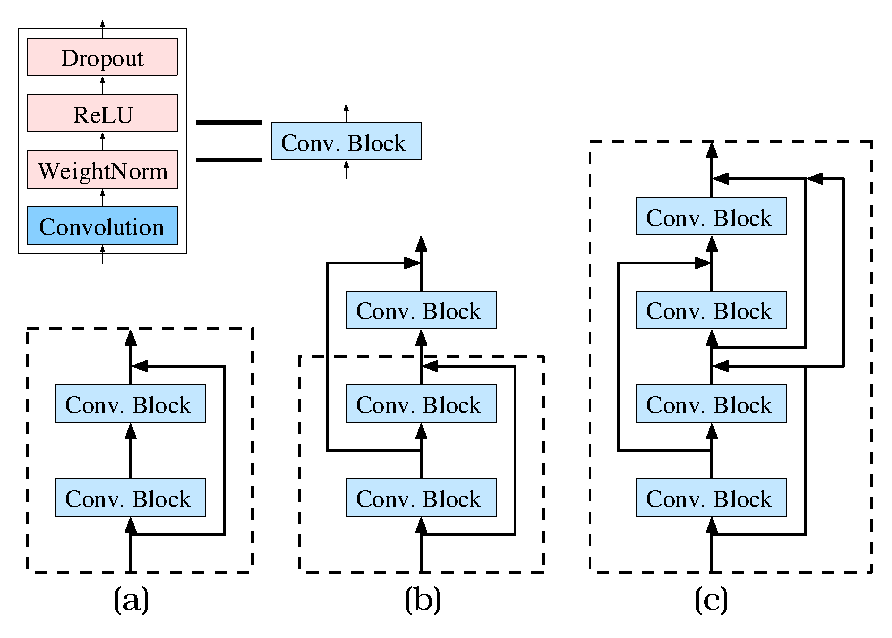
\includegraphics[width=10cm]{figGraph.eps}
  \vspace{-8pt}
  \captionof{figure}{\footnotesize{The original (a) Single and the proposed (b) Double and (c) Radical residual blocks. Lines in bold represent identity connections.} } 
  \label{figTCNGraph}
\end{center}
\end{minipage}
\end{center}


\vspace{-8pt}
\begin{center}
\begin{minipage}{\textwidth}
\begin{center}
  \includegraphics[width=11.5cm]{tcnmnistgraphs.png}
\begin{minipage}{0.9\textwidth}
\captionof{figure}{\footnotesize{A graph of the training losses, validation losses and the validation accuracy on SequenceMNIST as a function of the number of training iterations.}} 
\end{minipage}  
\end{center}
\end{minipage}
\end{center}



\vspace{-15pt}
\begin{minipage}{0.7\linewidth}
   \centering
   \label{tabseqmnist}
   \scalebox{1}{
   \begin{tabular}{c c c c}
    \hline
    Model & Test Acc. & Val. Acc. \\ \hline \hline
    TCN (Single) & \textbf{99.53\%} & 99.23\% \\ \hline
    TCN (Double) & 99.34\% & 99.07\% \\ \hline
    TCN (Radical) & 99.37\% & \textbf{99.30\%}  \\ \hline
    Dilated GRU \cite{dilatedgru} & 99.0\% & N/A  \\ \hline
    TCN (Original) \cite{tcn} & 99.0\% & N/A  \\ \hline
    \end{tabular}}
\end{minipage}
\begin{minipage}{0.25\linewidth}
\vspace{10pt}
\captionof{table}{\footnotesize{\textbf{SequenceMNIST}. A comparison with the current state of the art. Data not provided by the authors is marked as \textit{N/A}.} Best results are shown in bold.}
\end{minipage}
\vspace{-7pt}
\end{posterbox}












\begin{posterbox}[name=imagecaptioning,column=1,below=experiments]{Automatic Image Captioning}
We compared GRU and TCN models on the MSCOCO Captions \cite{mscoco} dataset. The models generate image captions by sequentially suggesting the next word in a sentence. Each word is represented as a one-hot vector encoding, and is given to the model through word embeddings.
\vspace{10pt}

A ResNet-18 \cite{resnet} was used to extract a 512-dimensional feature vector, describing a given image. The GRU initialized its first hidden layer with this vector, and both the TCN and GRU used it as a start of string token. Unknown words were replaced with the \textit{<UKN>} token, and the models stopped after predicting an end of string \textit{<EOS>} token. Let $S$ be the set of all predicted word probabilities $\hat{p}$, and $p$ the associated ground truth to word prediction $\hat{p}$. The total loss $L(\theta)$ which the models used is defined as:
\begin{equation}
L(\theta) = -\frac{1}{|S|} \sum_{p \in S} p \log{\hat{p}}
\end{equation}

\begin{center}
\begin{minipage}{\textwidth}
\begin{center}
  \includegraphics[width=11.5cm]{captionsnew.png}
\begin{minipage}{0.9\textwidth}
  \captionof{figure}{\footnotesize{Comparative results of the TCN and GRU automatic image annotation models on images from the MSCOCO Captions \cite{mscoco} validation dataset.}} 
  \label{figimagecaptioning}
\end{minipage}  
\end{center}
\end{minipage}
\end{center}

\vspace{-4pt}

\begin{minipage}{\linewidth}
\begin{center}
\label{tabimagecaptioning}
   \scalebox{0.795}{
   \begin{tabular}{c c c c c c c c}
    \hline
    Model & CIDEr-D & METEOR & Rouge-L & BLUE-1 & BLUE-2 & BLUE-3 & BLUE-4\\ \hline \hline
    TCN (C5) & 0.722 & 0.219& 0.482& 0.658& 0.476& 0.338& 0.240\\ \hline
    GRU (C5) & 0.741 & 0.222& 0.490& 0.668& 0.488& 0.347& 0.248\\ \hline
    \end{tabular}}
\begin{minipage}{0.9\textwidth}
\captionof{table}{\footnotesize\textbf{MSCOCO Results}. The TCN and GRU models evaluated on the automatic evaluation metrics of the MSCOCO test set evaluation server \cite{mscoco}.}
\end{minipage}  
\end{center}
\end{minipage}

\vspace{-7pt}

\begin{center}
\begin{minipage}{\textwidth}
\begin{center}
  \includegraphics[width=11.5cm]{tcngraphs.png}
\begin{minipage}{0.9\textwidth}
  \captionof{figure}{\footnotesize{A graph of the training and validation losses of the TCN and GRU models on the MSCOCO Captions \cite{mscoco} training dataset.}} 
\end{minipage}
\end{center}
\end{minipage}
\end{center}
\vspace{-20pt}
\end{posterbox}

















\begin{posterbox}[name=conclusion,column=1,below=imagecaptioning, above=bottom]{Conclusion}
The new suggested zero-padding and dilation scheme heavily outperformed the previous state of the art, halving the previous best test loss on SequenceMNIST. Regarding automatic image captioning, the TCN model differed by a higher quality of generated image captions and faster convergence speeds during training, despite a similarity of TCN and GRU performances on the automated evaluation metrics.%The TCN model is shown to generate image caption of higher quality and exhibits faster convergence speeds during training, despite a similarity of TCN and GRU performances on the automated evaluation metrics.
\end{posterbox}











\end{poster}
\end{document}
